

%% La classe stageM2R s'appuie sur la classe memoir, plus d'information sur le paquet: http://www.ctan.org/pkg/memoir
%% option possible de la classe stageM2R
% utf8  -> encodage du texte UTF8 (défaut: Latin1)
% final -> mode rapport de stage final (défaut: mode étude bibliographique)
% private -> indique une soutenance privée (défaut: soutenance publique)
\documentclass[utf8]{stageM2R} %-> etude bibliographique
%\documentclass[utf8,final]{stageM2R} %-> rapport final

\usepackage[style=numeric,citestyle=numeric,backend=bibtex]{biblatex}
\usepackage{wrapfig}
\usepackage{hhline}
\usepackage{subcaption}
\usepackage[]{algorithm2e}
\usepackage{amsthm}
\usepackage{mathtools}
\usepackage{float}

\bibliography{../../articles/biblio.bib}

\newcommand*{\addheight}[2][.5ex]{%
  \raisebox{0pt}[\dimexpr\height+(#1)\relax]{#2}%
}

%%%%%%%%%%%%%%%%%%%%%%%%%%%%
%%% Déclaration du stage %%%
%%%%%%%%%%%%%%%%%%%%%%%%%%%%

%% auteur
\author{Noé Le Philippe}
%% encadrants
\supervisor{William Puech}
%% lieu du stage (Optionnel)
\location{Équipe ICAR - LIRMM UM5506 - CNRS, Université de Montpellier}
%% titre du stage
\title{La phylogénie des images dans les réseaux sociaux} 
%% parcours du master
\track{IMAGINA}  
%% date de soutenance (Optionnel)
\date{\today} 
%% version du rapport (Optionnel)
\version{1}
%% Résumé en francais
\abstractfr{
Ce stage de master.
}
%% Résumé en anglais
\abstracteng{
  This master thesis.
}



\begin{document}   
%\selectlanguage{english} %% --> turn the document into english mode (Default is french)
\selectlanguage{french} 
\frontmatter  %% -> pas de numérotation numérique
\maketitle    %% -> création de la page de garde et des résumés
\cleardoublepage   
\tableofcontents %% -> table des matières
\mainmatter  %% -> numérotation numérique


%%%%%%%%%%%%%%%%%%%%%%%%%%%%%%
%%%%   DEBUT DU RAPPORT   %%%%
%%%%%%%%%%%%%%%%%%%%%%%%%%%%%%

\chapter{Introduction}
La phylogénie, en sciences naturelles, est définie\cite{phylogeny} comme l'étude des relations de parenté entre êtres vivants. Et c'est exactement de cela qu'il s'agit dans le cas des images, l'étude des relations de parenté entre images. \\
À l'ère des réseaux sociaux, il n'a jamais été aussi simple de partager des idées et du contenu. À chaque partage cependant, l'information peut être amenée à être modifiée. Les images, puisque c'est là notre sujet d'étude, peuvent avoir subi un certain nombre de transformations et modifications avant de nous parvenir. C'est dans ce contexte que nous allons intervenir, et tenter de reconstituer la phylogénie de l'image. Il peut être difficile de différentier cette image de l'originale, et de savoir laquelle est l'originale, mais c'est pourtant crucial dans un monde où l'information peut être falsifiée par tout le monde et extrêmement facilement. Les applications sont variées, et ne se cantonnent pas à la détection et la discrimination d'images altérées, on peut également se servir de la phylogénie de l'image pour optimiser de l'espace de stockage en ne gardant que l'originale ou encore suivre la diffusion et l'évolution des idées sur les réseaux sociaux.
\newpage

\section{Near-duplicate images (NDI)}
\label{subsec:ndi}
Nous travaillons sur un ensemble d'images, toutes similaires, et au milieu de cette jungle d'images, nous devons décider quelle image est le parent de quelle autre, ou autrement dit, quelles images sont des \textbf{near-duplicates}. Joly et al. \cite{joly2007content} définit la notion de near-duplicate comme suit : $I_{1} = T(I), T \in \mathcal{T}$ où $I$ est l'image parent, $I_{1}$ est l'image enfant et $\mathcal{T}$ est un ensemble de transformations autorisées, $I_{1}$ et $I$ sont alors des NDI. Dans le cas général, $\mathcal{T} = $ \textit{\{resampling, cropping, affine warping, color changing, lossy compression\}}, Fig. \ref{fig:near-duplicates-images} montre un exemple de near-duplicates, dans le cadre de ce stage cependant, $\mathcal{T} = $ \textit{\{lossy compression\}}. Notons l'utilisation du terme \textit{transformations autorisées}. Ce terme est double, d'une part, il place une limite arbitraire dans la force de la transformation, par exemple une image cropée à plus de 10\% pourra ne pas pas être considérée comme un near-duplicate, et d'autre part, il permet de restreindre l'espace des transformations possibles. Ainsi, dans le cadre du stage, seules les images de la troisième case de Fig. \ref{fig:near-duplicates-images} seront des NDI. Ces transformations peuvent évidemment se composer, et une image enfant peut être le résultat de plusieurs transformations.

\vspace{5mm}
\textbf{Note.} \textit{Nous utiliserons relation parent-enfant et relation de parenté de manière interchangeable dans le reste de ce rapport, mais c'est bien d'une relation parent-enfant qu'il s'agit.}

\begin{center}
\begin{figure}
\begin{tabular}{|c|c|c|}
      \hline
      \addheight{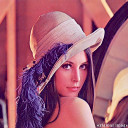
\includegraphics[width=23mm]{images/lena_base.jpg} 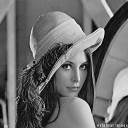
\includegraphics[width=23mm]{images/lena_bw.jpg}} &
      \addheight{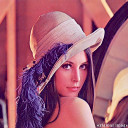
\includegraphics[width=23mm]{images/lena_base.jpg} 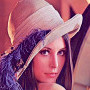
\includegraphics[width=23mm]{images/lena_crop.jpg}} &
      \addheight{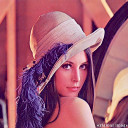
\includegraphics[width=23mm]{images/lena_base.jpg} 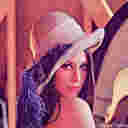
\includegraphics[width=23mm]{images/lena_comp.jpg}} \\
      \small couleur $\to$ noir et blanc & image entière $\to$ crop & image $\to$ image compressée\\
      \hline
\end{tabular}
\caption{Exemples de near-duplicates}
\label{fig:near-duplicates-images}
\end{figure}
\end{center}
\section{Arbre phylogénétique (Image Phylogeny Tree - IPT)}
C'est l'arbre représentant les relations de parenté entre les différentes images. Il sera extrait d'un ensemble de NDI, c'est l'objectif final de l'application. Un exemple est disponible Fig. \ref{fig:set-to-tree}. Le passage d'une génération à l'autre, autrement dit d'un noeud à son fils se fait à travers la transformation $I_{1} = T(I)$, ainsi, une image et son parent sont des NDI, alors qu'une images et ses soeurs ne le sont pas (Fig \ref{fig:tree-extract}).
\\ \indent
La reconstruction de l'arbre se concentre autour de deux problèmes principaux. Le premier est l'identification de la racine, et le second et l'estimation du reste de l'arbre. Il est en effet critique d'identifier correctement la racine. Prenons par exemple un des cas d'utilisation de l'IPT, la détection d'altération d'images. L'idée est que pour un ensemble d'images, plus on est proche de la racine, moins l'image a subi de transformations, et donc moins elle est altérée, avec dans le meilleur des cas, la racine en image originale. On voit bien que si on identifie mal la racine, on déduira, à tort, qu'une image n'a pas été altérée. Il n'est pas toujours garanti que la totalité des images de l'arbre original soit présente, de plus, certaines transformations peuvent être mineures, et difficile à détecter, c'est donc bien une estimation de l'arbre original qui sera faite.

\begin{figure}
  \begin{center}
    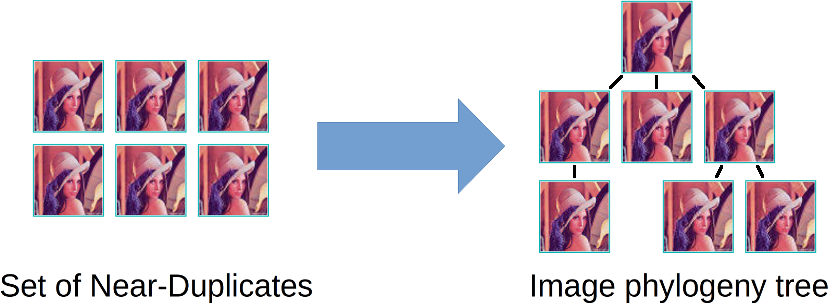
\includegraphics[width=120mm]{images/set_to_tree}
    \caption{Passage d'un ensemble de NDI à un arbre phylogénétique}
    \label{fig:set-to-tree}
  \end{center}
\end{figure}

\begin{figure}
  \begin{center}
    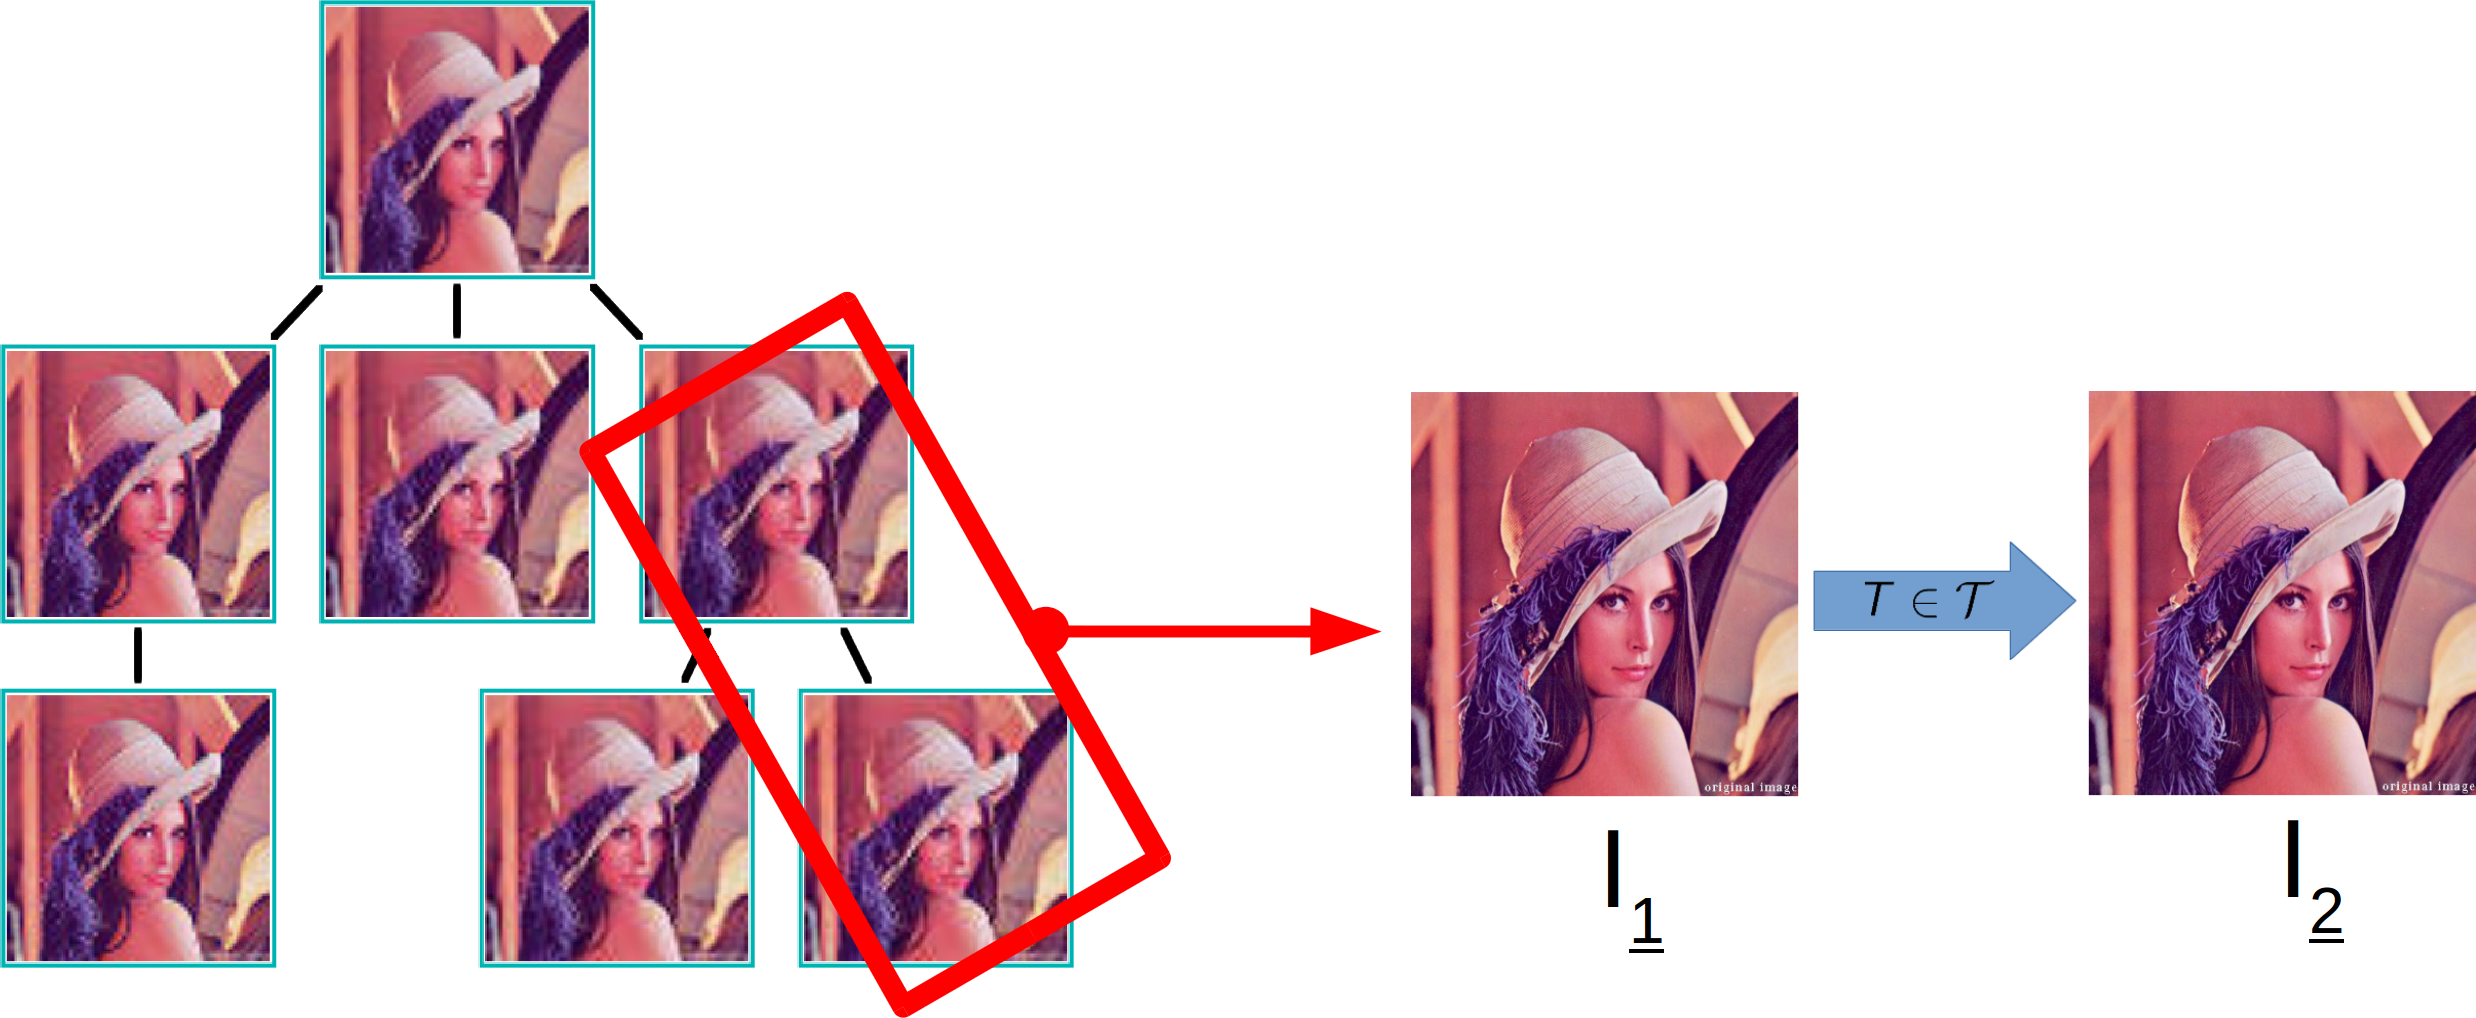
\includegraphics[width=120mm]{images/tree_extract}
    \caption{Passage d'une image parent à l'image enfant}
    \label{fig:tree-extract}
  \end{center}
\end{figure}

\section{Pourquoi se restreindre à la compression ?}
Comme mentionné précédemment, nous ne considérons que le cas de la compression avec perte en laissant de coté les autres transformations. Nous avons décidé de ne nous concentrer que sur une seule transformation pour avoir la possibilité de la traiter en détail et en profondeur dans le cadre du stage et ne pas devoir survoler sans approfondir toutes les transformations. Le choix de la compression est assez naturel, cela n'a, à notre connaissance, pas encore été traité dans le cadre le la phylogénie, et c'est un domaine largement étudié en forensic.

\chapter{État de l'art}
\section{Étude de l'arbre phylogénétique}
\subsection{La Visual Migration Map (VMM)}
C'est à notre connaissance, le premier article concernant vraiment notre sujet. Kennedy et al. \cite{kennedy2008internet} proposent une approche permettant d'automatiquement détecter la manière dont une image a été éditée ou manipulée, et d'en extraire des relations parent-enfant entre les images. Il vont construire à partir le l'estimation de ces transformations une Visual Migration Map (VMM) (voir Fig. \ref{vmm}) qui est en fait notre arbre de phylogénie.
\\ \indent
Ils partent du principe que les transformations sont directionnelles, c'est à dire que l'on de ne peut passer que d'une image moins transformée à une image plus transformée. Ainsi, ils vont tenter d'estimer la direction de chaque transformation entre deux images $I_{1}$ et $I_{2}$ (sachant que $\mathcal{T}$ = \textit{\{scaling, cropping, grayscale, overlay, insertion\}}). Trois scénarios sont alors possibles : si toutes les transformations sont dans le même sens, l'image fille est alors celle vers qui pointent les transformations, si les transformations sont dans des sens contraires, les images sont sûrement des soeurs, elles n'ont en tous cas pas de relation parent-enfant, et enfin si aucune transformation n'a été détectée, c'est que soit les images sont identiques, soit qu'elles ne sont pas des near-duplicates. On peut en voir un exemple Fig. \ref{vmm-directionnel}.
\\ \indent
Un graphe va ensuite être construit à partir des couples d'images pour lesquels une relation parent-enfant a été détectée. À noter qu'une relation parent-enfant ne veut pas forcément dire que c'est le parent direct mais plutôt un ancêtre. Ainsi, un noeud du graphe (une image) peut avoir plusieurs noeuds parents, pour finalement obtenir l'arbre désiré, seuls les chemins les plus longs sont conservés, comme on peut le voir Fig. \ref{vmm-tree}.

%%%%% parler de comment sont calculées les directions des transformations.
%%%%% parler des résultats ?
%%%%% parler de ce qui est bien dans cette méthode et de ce que l'on va utiliser.

% \begin{wrapfigure}{R}{0.5\textwidth}
%   \begin{center}
%     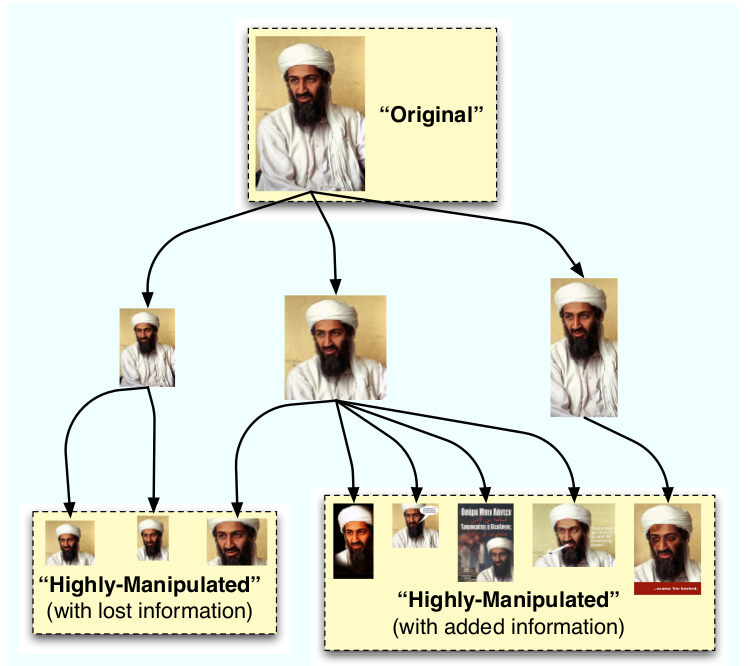
\includegraphics[width=0.48\textwidth]{images/vmm.png}
%   \end{center}
%     \label{vmm}
%     \caption{Exemple de VMM, tiré de \cite{internet}}
% \end{wrapfigure}

\begin{figure}
  \begin{center}
    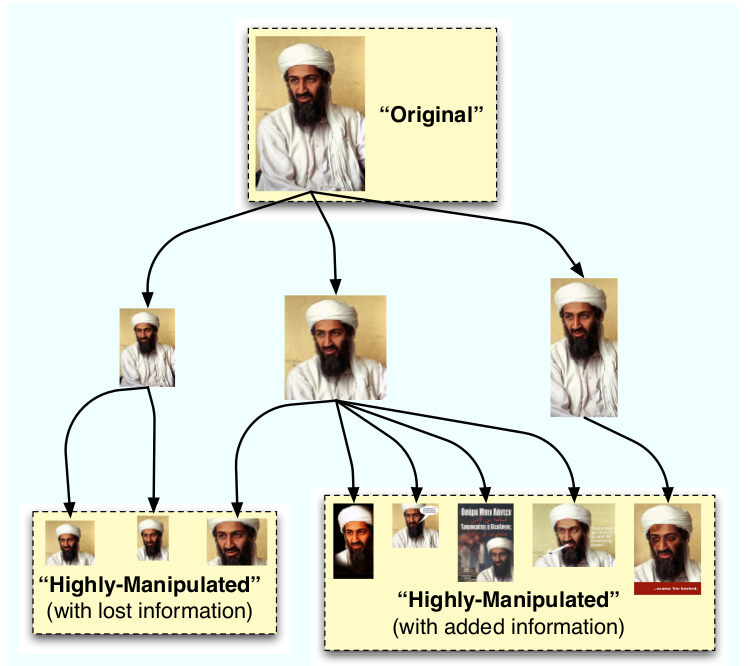
\includegraphics[width=70mm]{images/vmm.png}
    \caption{Exemple de VMM, issu de \cite{kennedy2008internet}}
    \label{vmm}
  \end{center}
\end{figure}

\begin{figure}
  \begin{center}
    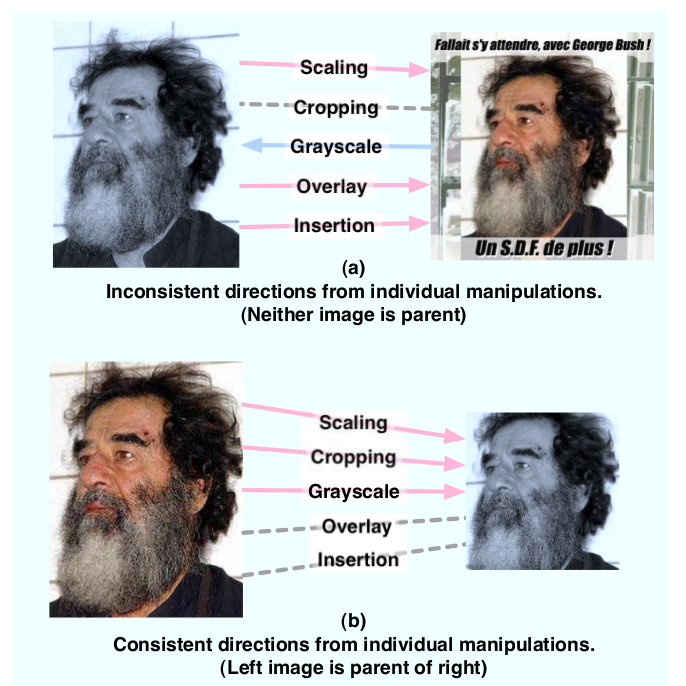
\includegraphics[width=70mm]{images/vmm_directionnel.png}
    \caption{Exemple de direction des transformations, issu de \cite{kennedy2008internet}}
    \label{vmm-directionnel}
  \end{center}
\end{figure}

\begin{figure}
  \begin{center}
    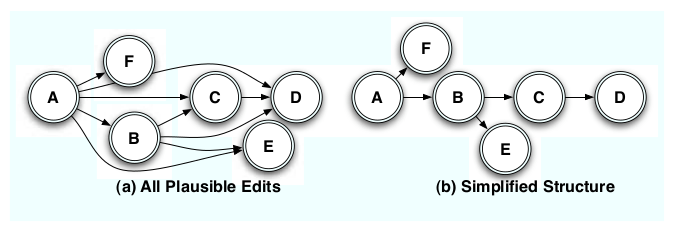
\includegraphics[width=100mm]{images/vmm_tree.png}
    \caption{Exemple de simplification de graphe, issu de \cite{kennedy2008internet}}
    \label{vmm-tree}
  \end{center}
\end{figure}

\subsection{Image Phylogeny Tree (IPT)}

Tout comme l'approche présentée précédemment, Dias et al. \cite{dias2010first}\cite{dias2012image} proposent une approche basée sur le contenu de l'image. Cela consiste a mapper une image sur le domaine d'une autre, pour pouvoir les comparer, et ensuite estimer le coût de cette opération, cela fait comme hypothèse que si deux images sont dépendantes, alors il est possible d'obtenir l'une en appliquant une transformation à l'autre. 

%%% proches = 
Les images sont comparées à l'aide d'une \textit{dissimilarity function d(.,.)} qui renvoie des petites valeurs lorsque les images sont proches (elles ont subi des transformations similaires). L'équation \ref{dissimilarity-function} détaille cette fonction. $A$ et $B$ sont les deux images qui vont être comparées, et $T_{\overrightarrow{\beta}} \in \mathcal{T}$ est la transformation en train d'être estimée. La transformation la plus faible est gardée comme résultat, c'est la transformation la plus probable qu'a pu subir l'image. À noter que $d(.,.)$ est asymétrique, c'est à dire que $d(A,B) \neq d(B,A)$, ce qui est parfaitement logique, en plus d'être nécessaire, sachant que les transformation sont directionnelles, comme expliqué précédemment.

\begin{equation}
  d(A,B) = \underset{T_{\overrightarrow{\beta}}}{min}\left | B - T_{\overrightarrow{\beta}}(A) \right |_{comparison\ method}
  \label{dissimilarity-function}
\end{equation}

On voit donc bien que la problématique principale de cette méthode est de trouver une bonne méthode de comparaison. Les auteurs procèdent de la manière suivante : 
\begin{itemize}
  \item Trouver des points caractéristiques (SURF \cite{bay2008speeded})
  \item Filtrer les points et estimer les paramètres de transforamtion affines tels que les translations, rotations, rééchantillonages... avec RANSAC \cite{ransac}
  \item Calculer la moyenne et la variance de chaque canal couleur de B pour normaliser les couleurs de A
  \item Compresser les résultats des deux étapes précédentes avec la table de quantification de B
\end{itemize}

La dissimilarité entre les deux images est enfin obtenue en utilisant la \textit{minimum squared error} (MSE) entre les deux images dans le domaine spatial comme technique de comparaison pour Équation \ref{dissimilarity-function}.

Ces quatre étapes ont servi à rendre les images comparables, en mappant l'une dans le domaine de l'autre, pour avoir des résultats pertinents.
%%%% Analyser leur méthode et ne pas simplement la décrire ?
% \vspace{3mm}
\paragraph{}

$d(.,.)$ est donc appliquée à tous les couples d'images de l'ensemble, pour créer une \textit{dissimilarity matrix}, une matrice de taille $n\times n$ qui sera ensuite donnée comme entrée à leur algorithme de reconstruction d'arbre, Oriented Kruskal. Nous n'allons pas entrer dans les détails de cet algorithme, il est expliqué de manière exhaustive dans \cite{dias2012image}, et ayant une approche différente (Chap. \ref{chap:notre_approche}), la reconstruction sera également différente.
% \vspace{3mm}
\paragraph{}                    

En plus de proposer une approche pour reconstituer l'arbre de phylogénie, ils proposent une approche pour comparer deux arbres, et donc évaluer notre arbre reconstruit si on le compare avec la vérité terrain. Cela consiste en quatre métriques : \\
\renewcommand{\arraystretch}{2}
\begin{tabular}{ll}
  \textbf{Root} & $
                  R(IPT_{1}, IPT_{2}) = $
                  \scalebox{0.65}{%
                  $
                  \begin{cases}
                    1 & if\ \texttt{Root(IPT}_{1}) = \texttt{Root(IPT}_{2}) \\
                    0 & Otherwise
                  \end{cases}
                        $} \\
  \textbf{Edges} & $E(IPT_{1}, IPT_{2}) = \frac{|E_{1} \cap E_{2}|} {n - 1}$ \\
  \textbf{Leaves} & $L(IPT_{1}, IPT_{2}) = \frac{|L_{1} \cap L_{2}|} {|L_{1} \cup L_{2}|}$ \\
  \textbf{Ancestry} & $A(IPT_{1}, IPT_{2}) = \frac{|A_{1} \cap A_{2}|} {|A_{1} \cup A_{2}|}$
\end{tabular}
\renewcommand{\arraystretch}{1.}
% \vspace{5mm}
\paragraph{}

\textbf{Root} est triviale, et renvoie si les racines sont identiques. \textbf{Edges} mesure le ratio de noeuds ayant le bon parent, \textbf{Leaves} est le ratio de feuilles correctes, et enfin \textbf{Ancestry} est le ratio d'ancêtres corrects jusqu'à la racine.

Ces métriques serviront à évaluer nos résultats dans la suite du stage.

\section{Analyse des recompression JPEG}
Notre but n'est pas vraiment de détecter si une image a été compressée plusieurs fois, nous sommes en effet quasi-certains que nos images auront été recompressées, puisque c'est précisément sur cela que nous travaillons, un ensemble de NDI, où $\mathcal{T} = {\{lossy\ compression\}}$. L'important est plutôt de savoir combien de fois, et à partir de qui l'image a été compressée, et donc pouvoir en déduire sa distance à la racine. La majorité des articles dans le domaine du forensic ne se concentrent que sur une image, pour en extraire le maximum d'informations possible. Ce n'est pas exactement notre cas, puisque les informations pertinentes pour nous ne sont pas dans l'image directement, mais plutôt dans ses relations avec les autres. Il nous a cependant paru important de traiter l'aspect forensic du problème, et se renseigner sur les différentes techniques, qui bien que créées pour un autre cas d'utilisation, peuvent, sinon s'adapter, au moins nous donner des pistes.

\subsection{Qu'est ce que JPEG ?}
Une rapide introduction sur ce qu'est le JPEG et son fonctionnement s'impose, nous ne parlerons cependant que du mode de compression avec perte, en laissant de coté son mode de compression sans perte, peu intéressant en plus de n'être virtuellement jamais utilisé. Pour de plus amples détails, le lecteur se dirigera vers \cite{wallace1992jpeg}.

\begin{figure}[H]
  \begin{center}
    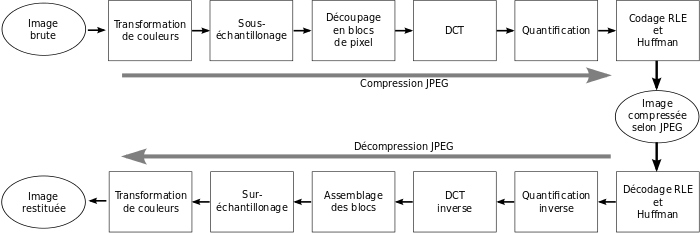
\includegraphics[width=120mm]{images/jpeg.png}
    \caption{Étapes de compression et décompression, issu de \cite{jpeg}}
    \label{fig:jpeg}
  \end{center}
\end{figure}

Fig. \ref{fig:jpeg} liste toutes les étapes permettant de passer d'une image non compressée à une image compressée pour finir par la décompresser, mais les étapes sont sommairement : 

\begin{itemize}
  \item L'image est convertie dans l'espace YUV
  \item Les canaux U et V sont sous-échantillonés
  \item Chaque canal est découpé en blocs de 8$\times$8
  \item Une DCT est appliquée à chacun de ces blocs
  \item Chaque coefficient est quantifié selon la table de quantification (voir Fig. \ref{fig:quantization_table}) correspondant au facteur de qualité Q $\in$ \textit{\{1,2,3,...,100\}} et arrondi
  \item Le tout est ensuite compressé à l'aide d'un codage entropique
\end{itemize}

C'est surtout l'étape de quantification qui va réduire la quantité d'information, et permettre de réduire la taille du fichier. Cette quantification, si elle est trop agressive va faire apparaitre des artefacts de bloc, des blocs 8$\times$8 visibles (voir Fig. \ref{fig:blocs_artefacts}). C'est ce qui caractérise le JPEG, et qui permet de détecter un certain nombres de choses, comme l'altération d'image \cite{bianchi2012image}, les doubles compressions \cite{bianchi2012detection} ou encore dans notre cas les relations de parenté.

\begin{figure}[H]
  \begin{center}
    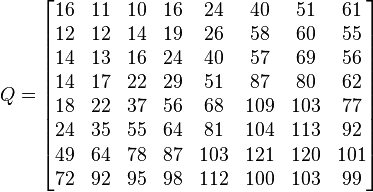
\includegraphics[width=60mm]{images/quantization_table.png}
    \caption{Exemple de table de quantification, issu de \cite{jpeg}}
    \label{fig:quantization_table}
  \end{center}
\end{figure}

\begin{figure}[H]
  \begin{center}
    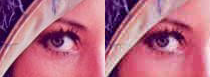
\includegraphics[width=120mm]{images/eyes.png}
    \caption{Artefacts de blocs, à gauche avec Q=90, à droite avec Q=20}
    \label{fig:blocs_artefacts}
  \end{center}
\end{figure}


\subsection{Détection des recompressions JPEG}
% La plupart des appareils photos aujourd'hui utilisent la compression JPEG pour compresser leurs images. 
% Le but dans la détection n'est pas simplement de savoir si l'image a 
\cite{feng2010jpeg}

\subsection{Détection des double compressions JPEG avec la même matrice de quantification}
\cite{huang2010detecting}


\subsection{Convergence des blocs lors de compressions successives}
L'intérêt de la méthode proposée par \citeauthor{CarneinSB2016TelltaleWatermarks} \cite{CarneinSB2016TelltaleWatermarks} est l'estimation du nombre de compression JPEG qu'a pu subir l'image, une estimation qui va au-delà de deux ou trois compression successives \cite{huang2010detecting}\cite{}, il est en effet possible d'aller jusqu'à plusieurs centaines de compressions. Cette approche se base sur la notion de blocs cycliques.

Lors de compressions successives, une phénomène appelé \textit{convergence de bloc} peut être observé. Un bloc converge lorsque la valeur des pixels du bloc à la compression $t$ est égale à la valeurs des pixels à la compression $t + 1$, ce bloc est alors appelé stable \cite{lai2013block}. Certains blocs cependant échappent à cet effet et exhibe un phénomène de cycle. C'est à dire que $valeur\ des\ pixels(t) = valeur\ des\ pixels(t + n), n > 1$.

Ces blocs sont nommés blocs compteurs. Ainsi, si un bloc de l'image a un cycle de longueur $l=9$, on pourra savoir, modulo $l$, combien de compressions a subi l'image. Et avec plus de blocs, ayant chacun des $l$ différents, il est possible d'aller bien plus loin dans le nombre de compressions. Prenons l'exemple de trois blocs pour lesquels $l_{1} = 2$, $l_{2} = 5$ et $l_{3} = 9$. Le nombre maximum de compressions successives que l'on pourra estimer est le \textit{plus petit commun multiple} des ces longueurs, autrement dit, $ppcm(2, 5, 9) = 90$, soit 90 compressions successives, et pour l'exemple Fig. \ref{fig:insertion_blocs}, $ppcm(6, 7, 10, 12) = 420$.

\paragraph{}
Les auteurs proposent deux approches pour les blocs cycliques. La première est de détecter les blocs cyliques à l'aide d'une recherche exhaustive sur l'ensemble des blocs et un certain nombre de compressions puis sélectionner les blocs intéressants. Cette méthode, bien qu'étant la plus simple, et ne modifiant pas l'image, peut cependant rencontrer des problèmes lorsqu'elle comporte un grand nombre de blocs plats, des blocs ayant tous les pixels de la même valeur, ces blocs ne peuvent en effet pas être des blocs cycliques, et il peut alors être difficile de trouver des blocs ayant des cycles de longueur intéressante. La deuxième approche proposée est donc d'insérer des blocs artificiellement créés dans l'image (voir Fig. \ref{fig:insertion_blocs}). 

Cette méthode nécessite de prendre un certain nombre de précaution et requiert une protection (padding) autour des blocs insérés. L'algorithme de sur-échantillonage est en effet parfois amené à utiliser les valeurs des pixels des blocs adjacents pour un meilleur rendu et provoquer un effet de débordement (spill over) des valeurs \cite{carnein2015forensics}, ce qui modifie le bloc artificiellement créé (dans le vide) et donc modifie son cycle, rendant nulle son information.

\begin{figure}
  \begin{center}
    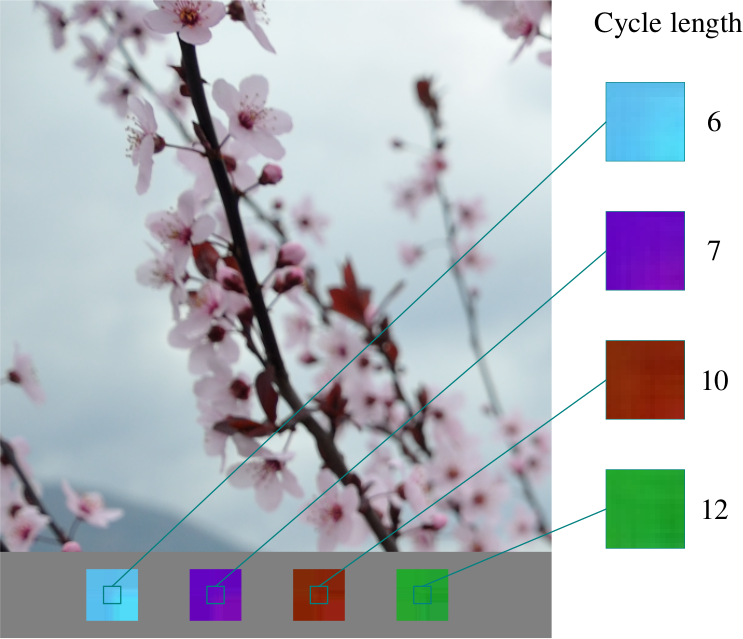
\includegraphics[width=80mm]{images/insertion_blocs}
    \caption{Exemple d'insertion de blocs, issu de \cite{CarneinSB2016TelltaleWatermarks}}
    \label{fig:insertion_blocs}
  \end{center}
\end{figure}


%%%%parler du calcul des blocs et tout
\paragraph{}

Le principal inconvénient de cette méthode, si on utilise les blocs de l'image, et qu'on laisse de coté l'insertion de blocs, est qu'elle se restreint à des images ayant toutes le même facteur de qualité, et en particulier $Q = 100$, pour lequel les cycles sont les plus longs, et donc donnent le plus d'informations. C'est un cas trop spécifique pour notre cadre d'utilisation : les réseaux sociaux, où les facteurs de qualité de compression varient en fonction de l'application utilisée. Cette méthode est en effet plus orientée vers le tatouage et le tracage d'images, et est la plus simple à utiliser lorsque l'on a, à un moment, été en possession de l'image originale et pris soin de noter les blocs intéressants.

\section{Distances entre distributions}
\cite{oikawa2015distances}

\chapter{Notre approche}
\label{chap:notre_approche}
\section{Principe}

% \fbox{
%   \parbox{\textwidth}{
%     \underline{Énoncé} :\\
%     Pour tout couple d'image (A, B), s'il n'est pas possible de prouver que A n'est pas le parent de B, alors il y a une relation parent-enfant entre A et B, A $\to$ B.
%   }
% }
% \\ \\ 
% \fbox{
%   \parbox{\textwidth}{
%     \underline{Preuve (empirique)} :\\
%     Si une fonction détecte à chaque fois qu'il est présent un marqueur prouvant qu'il n'y a pas de relation de parenté entre deux images, alors s'il n'en détecte pas c'est qu'il y a une relation de parenté entre les deux images.
%   }
% }

\newtheorem*{parentage}{Théorème}
\begin{parentage}
  Pour tout couple d'image (A, B), s'il n'est pas possible de prouver que A n'est pas le parent de B, alors il y a une relation parent-enfant entre A et B, A $\to$ B.
\end{parentage}

\begin{proof}
  Soit $f(A,B)$ une fonction qui pour tout couple d'image $(A, B)$ détecte à chaque qu'il est présent un marqueur prouvant qu'il n'y a pas de relation de parenté entre $A$ et $B$. Si $f(A,B)$ ne détecte rien alors c'est que A est le parent de B.
\end{proof}

\section{La construction de l'arbre}
On va ainsi pour tout couple d'image de notre ensemble tenter de nier qu'il existe une relation de parenté, cela va permettre d'extraire une matrice binaire, de la taille de l'ensemble d'image, où une case à vrai indiquera une relation de parenté. À noter une fois de plus que ce n'est pas forcément un parent direct mais plutôt un ancêtre. \\ \indent
On peut noter plusieurs choses intéressantes de l'exemple Fig. \ref{parentage_tree}. L'image $I_{2}$ a toute sa colonne marquée à vrai, c'est à dire que c'est un parent commun à toutes les autres images, et sa ligne n'a que des 0, elle n'a donc aucun parent. On se sert de ce principe pour la reconstruction de l'arbre à partir de la matrice : une image qui n'a pas de parent est la racine. On peut également remarquer les colonnes où toutes les cases sont à 0, cela veut dire que ces images ne sont le parent de personne, et donc sont des feuilles.

\begin{figure}
  \begin{subfigure}{.5\textwidth}
    \centering
    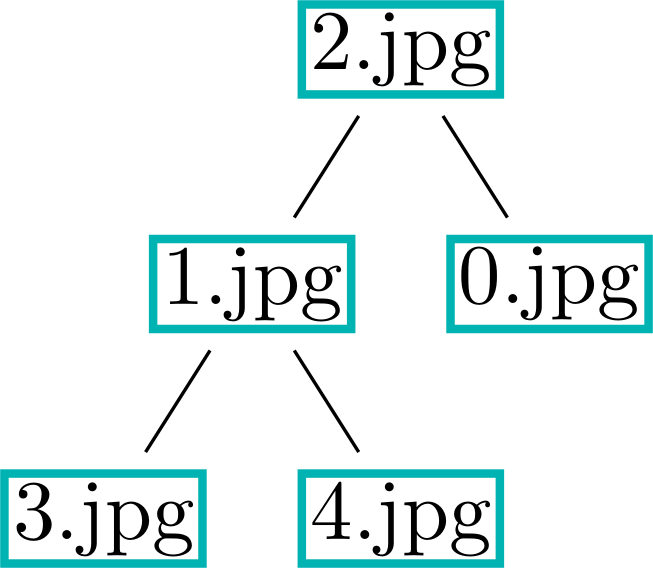
\includegraphics[width=.5\linewidth]{images/algo_tree.png}
    \caption{Arbre de phylogénie}
    \label{algo_tree}
  \end{subfigure}%
  \begin{subfigure}{.5\textwidth}
    \centering
    \begin{tabular}{|r||c|c|c|c|c|}
      - & $I_{0}$ & $I_{1}$ & $I_{2}$ & $I_{3}$ & $I_{4}$ \\ \hhline{|=::=|=|=|=|=|}
      $I_{0}$ & - & 0 & 0 & 0 & 0 \\ \hline
      $I_{1}$ & 0 & - & 0 & 1 & 1 \\ \hline
      $I_{2}$ & 1 & 1 & - & 1 & 1 \\ \hline
      $I_{3}$ & 0 & 0 & 0 & - & 0 \\ \hline
      $I_{4}$ & 0 & 0 & 0 & 0 & - \\ \hline
    \end{tabular} 
    \caption{Matrice de parenté}
    \label{parentage_matrix}
  \end{subfigure}
  \caption{Une arbre de phylogénie et sa matrice de parenté}
  \label{parentage_tree}
\end{figure}

\subsection{L'algorithme de reconstruction}
De ces quelques principes nous avons extrait un algorithme. \vspace{5mm}

\begin{algorithm}[H]
  \LinesNumbered
  \KwData{M a n$\times$n parentage matrix}
  \KwResult{the root of the tree}
  \BlankLine
  $nextRoot \leftarrow$ row with min sum of elements\;
  $treeRoot \leftarrow nextRoot$\;
  \BlankLine

  \ForAll{rows row of M}{
    $root \leftarrow nextRoot$\;
    mark $root$ as done\;
    \BlankLine
    \For{$i\leftarrow 0$ \KwTo n}{
      $row[i] \leftarrow 0$\;
      \If{sum of elements of row == 0} {
        add $i$ as child of $root$\;
      }
      \If{row has the smallest sum of elements and is not marked as done} {
        $nextRoot \leftarrow i$\;
      }
    }
  }
  \KwRet treeRoot
\end{algorithm}
\vspace{5mm}

Il prend en entrée la matrice de parenté détaillée précédemment et retourne la racine de l'arbre. La philosophie de l'algorithme est qu'une image n'ayant aucun parent est la racine, et ce de manière récursive grâce à la structure d'arbre.

% La ligne 1 marque $nextRoot$ comme la ligne avec la plus petite somme des éléments, étant une matrice binaire, où les valeurs sont 0 et 1, c'est donc l'image qui a le moins de parent, autrement dit la racine.

% La ligne 5 marque $root$ comme terminée, c'est pour ne la traiter qu'une fois, en effet, dans un arbre, il n'y a pas de cycle, on ne peut donc pas 
% La condition lignes 8-10 ajoute l'image à l'indice $i$ comme enfant de $root$. La condition d'avoir tous les éléments de la ligne à 0, c'est à dire de n'avoir plus aucun parent

À chaque tour de boucle, une image est sélectionnée comme la racine (lignes 1 et 11) et nommée $root$, elle est retirée (ligne 7) des ancêtres des autres images si c'est un ancêtre. Si ces autres images n'ont plus d'ancêtre (ligne 8), c'est que $root$ était le parent direct de l'image en train d'être traitée, cette image est donc ajoutée comme enfant de $root$ (ligne 9). La ligne 5 permet de ne traiter qu'une fois chaque image comme racine potentielle.

Cet algorithme a une complexité de $O(n^{2})$. Il y a deux boucles imbriquées, et si les sommes sont calculées une une seule fois au début et mises à jour à chaque fois qu'un parent est enlevé, il n'y a pas de boucle supplémentaire augmentant la complexité.

Le but est donc de trouver la fonction permettant de détecter le marqueur prouvant qu'il n'y a pas de parenté. 
% Et même si cette fonction n'est pas parfaite, et qu'elle se trompe dans ses prédictions, l'algorithme est robuste et premet tout de même d'obtenir des résultats cohérents si on s'appuie sur les métriques introduites pas \cite{dias2010first} pour évaluer l'arbre (voir Fig. \ref{algo-robuste}).

Il nous a semblé important, même dans le cadre de l'étude bibliographique, d'élaborer cet algorithme. Il est en effet assez simple mais néanmoins indispensable à notre méthode, et aurait pu orienter différemment nos recherche et notre méthode s'il n'avait pas été imaginé. Le reste du stage sera consacré à élaborer la fonction énoncée précédemment, et c'est là que la majorité du travail se concentrera.

Cette approche a pour avantage de réduire l'évaluation d'un arbre de phylogénie à partir d'un ensemble d'images à l'évaluation binaire de parenté entre deux images.

%%%% faire une trace de l'algo %%%%%
\chapter{Conclusion}

% \nocite{*}
\printbibliography

\end{document}

    
%%% Local Variables: 
%%% mode: latex
%%% TeX-master: t
%%% End:  
 